\documentclass[a4paper]{book}
\usepackage{makeidx}
\usepackage{natbib}
\usepackage{graphicx}
\usepackage{multicol}
\usepackage{float}
\usepackage{listings}
\usepackage{color}
\usepackage{ifthen}
\usepackage[table]{xcolor}
\usepackage{textcomp}
\usepackage{alltt}
\usepackage{ifpdf}
\ifpdf
\usepackage[pdftex,
            pagebackref=true,
            colorlinks=true,
            linkcolor=blue,
            unicode
           ]{hyperref}
\else
\usepackage[ps2pdf,
            pagebackref=true,
            colorlinks=true,
            linkcolor=blue,
            unicode
           ]{hyperref}
\usepackage{pspicture}
\fi
\usepackage[utf8]{inputenc}
\usepackage{mathptmx}
\usepackage[scaled=.90]{helvet}
\usepackage{courier}
\usepackage{sectsty}
\usepackage[titles]{tocloft}
\usepackage{doxygen}
\lstset{language=C++,inputencoding=utf8,basicstyle=\footnotesize,breaklines=true,breakatwhitespace=true,tabsize=8,numbers=left }
\makeindex
\setcounter{tocdepth}{3}
\renewcommand{\footrulewidth}{0.4pt}
\renewcommand{\familydefault}{\sfdefault}
\hfuzz=15pt
\setlength{\emergencystretch}{15pt}
\hbadness=750
\tolerance=750
\begin{document}
\hypersetup{pageanchor=false,citecolor=blue}
\begin{titlepage}
\vspace*{7cm}
\begin{center}
{\Large \-My \-Project }\\
\vspace*{1cm}
{\large \-Generated by Doxygen 1.7.6.1}\\
\vspace*{0.5cm}
{\small Sat Mar 22 2014 18:25:52}\\
\end{center}
\end{titlepage}
\clearemptydoublepage
\pagenumbering{roman}
\tableofcontents
\clearemptydoublepage
\pagenumbering{arabic}
\hypersetup{pageanchor=true,citecolor=blue}
\chapter{\-Class \-Index}
\section{\-Class \-Hierarchy}
\-This inheritance list is sorted roughly, but not completely, alphabetically\-:\begin{DoxyCompactList}
\item \contentsline{section}{\-Abstract\-Cache}{\pageref{classAbstractCache}}{}
\begin{DoxyCompactList}
\item \contentsline{section}{\-F\-I\-F\-O\-Cache}{\pageref{classFIFOCache}}{}
\item \contentsline{section}{\-L\-M\-U\-Cache}{\pageref{classLMUCache}}{}
\item \contentsline{section}{\-L\-R\-U\-Cache}{\pageref{classLRUCache}}{}
\item \contentsline{section}{\-Random\-Cache}{\pageref{classRandomCache}}{}
\end{DoxyCompactList}
\item \contentsline{section}{\-R\-P\-C\-Proxy\-Handler}{\pageref{classRPCProxyHandler}}{}
\item \contentsline{section}{\-U\-R\-L\-Node}{\pageref{classURLNode}}{}
\end{DoxyCompactList}

\chapter{\-Class \-Index}
\section{\-Class \-List}
\-Here are the classes, structs, unions and interfaces with brief descriptions\-:\begin{DoxyCompactList}
\item\contentsline{section}{\hyperlink{classAbstractCache}{\-Abstract\-Cache} }{\pageref{classAbstractCache}}{}
\item\contentsline{section}{\hyperlink{classFIFOCache}{\-F\-I\-F\-O\-Cache} \\*\hyperlink{classFIFOCache}{\-F\-I\-F\-O\-Cache} }{\pageref{classFIFOCache}}{}
\item\contentsline{section}{\hyperlink{classLMUCache}{\-L\-M\-U\-Cache} \\*\hyperlink{classLMUCache}{\-L\-M\-U\-Cache} }{\pageref{classLMUCache}}{}
\item\contentsline{section}{\hyperlink{classLRUCache}{\-L\-R\-U\-Cache} \\*\hyperlink{classLRUCache}{\-L\-R\-U\-Cache} }{\pageref{classLRUCache}}{}
\item\contentsline{section}{\hyperlink{classRandomCache}{\-Random\-Cache} \\*\hyperlink{classRandomCache}{\-Random\-Cache} }{\pageref{classRandomCache}}{}
\item\contentsline{section}{\hyperlink{classRPCProxyHandler}{\-R\-P\-C\-Proxy\-Handler} }{\pageref{classRPCProxyHandler}}{}
\item\contentsline{section}{\hyperlink{classURLNode}{\-U\-R\-L\-Node} }{\pageref{classURLNode}}{}
\end{DoxyCompactList}

\chapter{\-File \-Index}
\section{\-File \-List}
\-Here is a list of all documented files with brief descriptions\-:\begin{DoxyCompactList}
\item\contentsline{section}{\hyperlink{AbstractCache_8cpp}{\-Abstract\-Cache.\-cpp} }{\pageref{AbstractCache_8cpp}}{}
\item\contentsline{section}{\hyperlink{AbstractCache_8h}{\-Abstract\-Cache.\-h} }{\pageref{AbstractCache_8h}}{}
\item\contentsline{section}{\hyperlink{FIFOCache_8h}{\-F\-I\-F\-O\-Cache.\-h} }{\pageref{FIFOCache_8h}}{}
\item\contentsline{section}{\hyperlink{LRUCache_8h}{\-L\-R\-U\-Cache.\-h} }{\pageref{LRUCache_8h}}{}
\end{DoxyCompactList}

\chapter{\-Class \-Documentation}
\hypertarget{classAbstractCache}{\section{\-Abstract\-Cache \-Class \-Reference}
\label{classAbstractCache}\index{\-Abstract\-Cache@{\-Abstract\-Cache}}
}
\-Inheritance diagram for \-Abstract\-Cache\-:\begin{figure}[H]
\begin{center}
\leavevmode
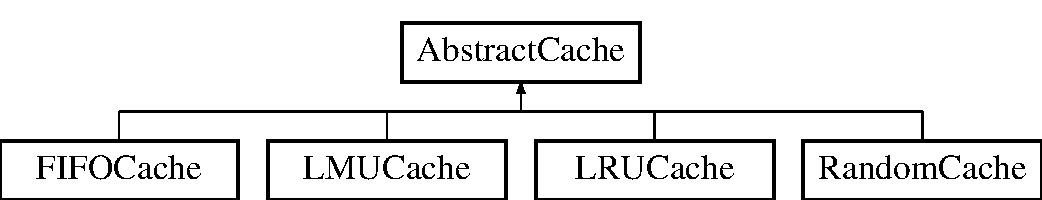
\includegraphics[height=2.000000cm]{classAbstractCache}
\end{center}
\end{figure}
\subsection*{\-Public \-Member \-Functions}
\begin{DoxyCompactItemize}
\item 
void \hyperlink{classAbstractCache_adcfda4aa5503e9ea60d2bc5575c04cd3}{insert\-Into\-Cache} (string url, string content)
\begin{DoxyCompactList}\small\item\em \-Insert \-Into \-Cache. \end{DoxyCompactList}\item 
void \hyperlink{classAbstractCache_a7cba328082bcd2f8a02e52546b9dd244}{delete\-From\-Cache} ()
\begin{DoxyCompactList}\small\item\em \-Delete \-Web \-Content \-From \-Cache. \end{DoxyCompactList}\item 
string \hyperlink{classAbstractCache_a9b49b5835bbe2fa878bac959ebbec925}{get\-From\-Cache} (string url)
\begin{DoxyCompactList}\small\item\em \-Get \-Web \-Content from \-Cache. \end{DoxyCompactList}\item 
\hypertarget{classAbstractCache_a0b8d729d097b1726cb01fa8d35a25e62}{void {\bfseries set\-Max\-Cache\-Size} (long size)}\label{classAbstractCache_a0b8d729d097b1726cb01fa8d35a25e62}

\item 
\hypertarget{classAbstractCache_a67552fbca85ce7dbc7e2c553b1036884}{virtual void {\bfseries update\-List} (string url)=0}\label{classAbstractCache_a67552fbca85ce7dbc7e2c553b1036884}

\item 
\hypertarget{classAbstractCache_ae9fe168b0b9167c27b94b4a3a1be788c}{virtual int {\bfseries pick\-Index\-For\-Next\-Deletion} ()=0}\label{classAbstractCache_ae9fe168b0b9167c27b94b4a3a1be788c}

\item 
\hypertarget{classAbstractCache_a910756174d1ee21eac16a4be3f7c881a}{virtual void {\bfseries insert\-Into\-List} (string url, string content)=0}\label{classAbstractCache_a910756174d1ee21eac16a4be3f7c881a}

\end{DoxyCompactItemize}
\subsection*{\-Public \-Attributes}
\begin{DoxyCompactItemize}
\item 
\hypertarget{classAbstractCache_a5db4a215715082ca927f75fec6fe274c}{unsigned long {\bfseries max\-Cache\-Size}}\label{classAbstractCache_a5db4a215715082ca927f75fec6fe274c}

\item 
\hypertarget{classAbstractCache_a3b7d8e12031d428787a75852370631e2}{unsigned long {\bfseries cache\-Size}}\label{classAbstractCache_a3b7d8e12031d428787a75852370631e2}

\item 
\hypertarget{classAbstractCache_a4ee0357340f21b0989bc8764db0fabce}{unordered\-\_\-map$<$ string, string $>$ {\bfseries map}}\label{classAbstractCache_a4ee0357340f21b0989bc8764db0fabce}

\item 
\hypertarget{classAbstractCache_abe36acc627f10c65bfd04e3833011d7b}{vector$<$ \hyperlink{classURLNode}{\-U\-R\-L\-Node} $>$ {\bfseries list}}\label{classAbstractCache_abe36acc627f10c65bfd04e3833011d7b}

\end{DoxyCompactItemize}


\subsection{\-Member \-Function \-Documentation}
\hypertarget{classAbstractCache_a7cba328082bcd2f8a02e52546b9dd244}{\index{\-Abstract\-Cache@{\-Abstract\-Cache}!delete\-From\-Cache@{delete\-From\-Cache}}
\index{delete\-From\-Cache@{delete\-From\-Cache}!AbstractCache@{\-Abstract\-Cache}}
\subsubsection[{delete\-From\-Cache}]{\setlength{\rightskip}{0pt plus 5cm}void {\bf \-Abstract\-Cache\-::delete\-From\-Cache} (
\begin{DoxyParamCaption}
{}
\end{DoxyParamCaption}
)}}\label{classAbstractCache_a7cba328082bcd2f8a02e52546b9dd244}


\-Delete \-Web \-Content \-From \-Cache. 

\begin{DoxyReturn}{\-Returns}
none 
\end{DoxyReturn}
\hypertarget{classAbstractCache_a9b49b5835bbe2fa878bac959ebbec925}{\index{\-Abstract\-Cache@{\-Abstract\-Cache}!get\-From\-Cache@{get\-From\-Cache}}
\index{get\-From\-Cache@{get\-From\-Cache}!AbstractCache@{\-Abstract\-Cache}}
\subsubsection[{get\-From\-Cache}]{\setlength{\rightskip}{0pt plus 5cm}string {\bf \-Abstract\-Cache\-::get\-From\-Cache} (
\begin{DoxyParamCaption}
\item[{string}]{url}
\end{DoxyParamCaption}
)}}\label{classAbstractCache_a9b49b5835bbe2fa878bac959ebbec925}


\-Get \-Web \-Content from \-Cache. 


\begin{DoxyParams}{\-Parameters}
{\em \-U\-R\-L} & \\
\hline
\end{DoxyParams}
\begin{DoxyReturn}{\-Returns}
\-Web \-Content 
\end{DoxyReturn}
\hypertarget{classAbstractCache_adcfda4aa5503e9ea60d2bc5575c04cd3}{\index{\-Abstract\-Cache@{\-Abstract\-Cache}!insert\-Into\-Cache@{insert\-Into\-Cache}}
\index{insert\-Into\-Cache@{insert\-Into\-Cache}!AbstractCache@{\-Abstract\-Cache}}
\subsubsection[{insert\-Into\-Cache}]{\setlength{\rightskip}{0pt plus 5cm}void {\bf \-Abstract\-Cache\-::insert\-Into\-Cache} (
\begin{DoxyParamCaption}
\item[{string}]{url, }
\item[{string}]{content}
\end{DoxyParamCaption}
)}}\label{classAbstractCache_adcfda4aa5503e9ea60d2bc5575c04cd3}


\-Insert \-Into \-Cache. 


\begin{DoxyParams}{\-Parameters}
{\em url} & -\/ \-U\-R\-L \\
\hline
{\em \-Web} & \-Content \\
\hline
\end{DoxyParams}


\-The documentation for this class was generated from the following files\-:\begin{DoxyCompactItemize}
\item 
\hyperlink{AbstractCache_8h}{\-Abstract\-Cache.\-h}\item 
\hyperlink{AbstractCache_8cpp}{\-Abstract\-Cache.\-cpp}\end{DoxyCompactItemize}

\hypertarget{classFIFOCache}{\section{\-F\-I\-F\-O\-Cache \-Class \-Reference}
\label{classFIFOCache}\index{\-F\-I\-F\-O\-Cache@{\-F\-I\-F\-O\-Cache}}
}


\-F\-I\-F\-O \-Cache.  




{\ttfamily \#include $<$\-F\-I\-F\-O\-Cache.\-h$>$}

\-Inheritance diagram for \-F\-I\-F\-O\-Cache\-:\begin{figure}[H]
\begin{center}
\leavevmode
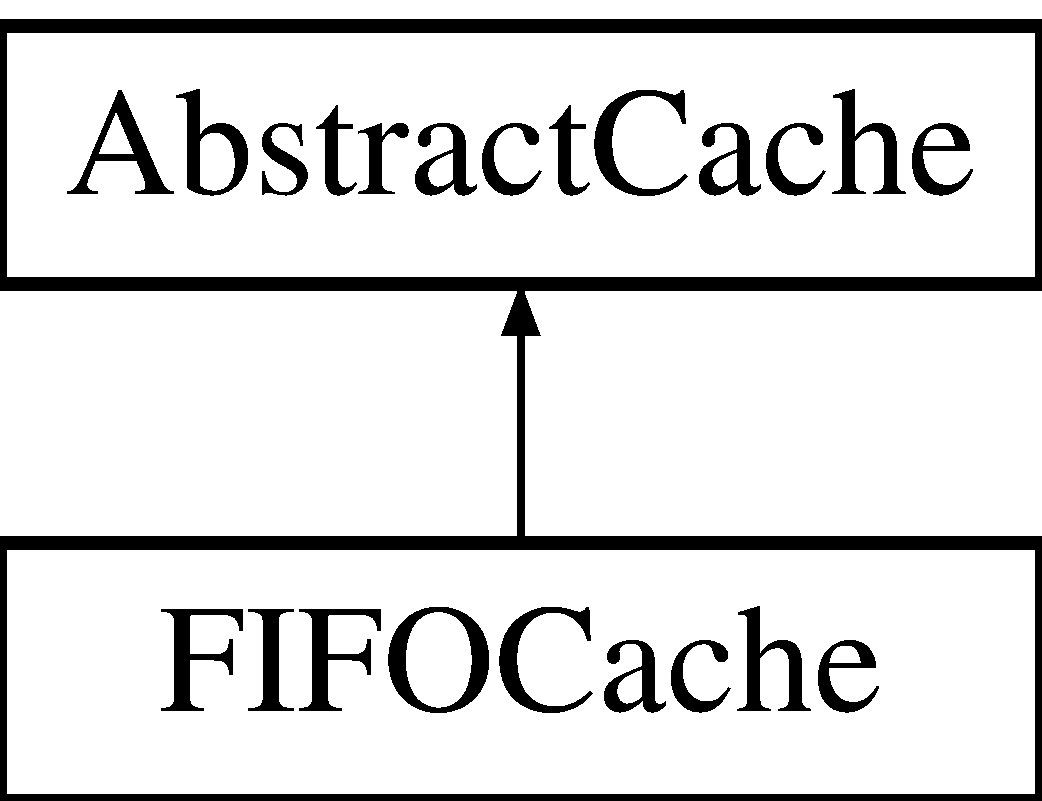
\includegraphics[height=2.000000cm]{classFIFOCache}
\end{center}
\end{figure}
\subsection*{\-Public \-Member \-Functions}
\begin{DoxyCompactItemize}
\item 
\hypertarget{classFIFOCache_a1ae7ca5adab1d06c341510f1f2fee299}{\hyperlink{classFIFOCache_a1ae7ca5adab1d06c341510f1f2fee299}{$\sim$\-F\-I\-F\-O\-Cache} ()}\label{classFIFOCache_a1ae7ca5adab1d06c341510f1f2fee299}

\begin{DoxyCompactList}\small\item\em \-Destructor. \end{DoxyCompactList}\item 
\hypertarget{classFIFOCache_a12486ada6ceb70c77f3cd4f40f295928}{\hyperlink{classFIFOCache_a12486ada6ceb70c77f3cd4f40f295928}{\-F\-I\-F\-O\-Cache} ()}\label{classFIFOCache_a12486ada6ceb70c77f3cd4f40f295928}

\begin{DoxyCompactList}\small\item\em \-Constructor. \end{DoxyCompactList}\item 
void \hyperlink{classFIFOCache_a73b7632a308ed4813d8c7e03cf597d47}{update\-List} (string url)
\begin{DoxyCompactList}\small\item\em \-Update the \-Queue. \end{DoxyCompactList}\item 
int \hyperlink{classFIFOCache_a16f6449563e0e83af7069406a14089e9}{pick\-Index\-For\-Next\-Deletion} ()
\begin{DoxyCompactList}\small\item\em \-Select next candidate entry for eviction. \end{DoxyCompactList}\end{DoxyCompactItemize}


\subsection{\-Detailed \-Description}
\-F\-I\-F\-O \-Cache. 

\subsection{\-Member \-Function \-Documentation}
\hypertarget{classFIFOCache_a16f6449563e0e83af7069406a14089e9}{\index{\-F\-I\-F\-O\-Cache@{\-F\-I\-F\-O\-Cache}!pick\-Index\-For\-Next\-Deletion@{pick\-Index\-For\-Next\-Deletion}}
\index{pick\-Index\-For\-Next\-Deletion@{pick\-Index\-For\-Next\-Deletion}!FIFOCache@{\-F\-I\-F\-O\-Cache}}
\subsubsection[{pick\-Index\-For\-Next\-Deletion}]{\setlength{\rightskip}{0pt plus 5cm}int {\bf \-F\-I\-F\-O\-Cache\-::pick\-Index\-For\-Next\-Deletion} (
\begin{DoxyParamCaption}
{}
\end{DoxyParamCaption}
)\hspace{0.3cm}{\ttfamily  \mbox{[}virtual\mbox{]}}}}\label{classFIFOCache_a16f6449563e0e83af7069406a14089e9}


\-Select next candidate entry for eviction. 

\begin{DoxyReturn}{\-Returns}
\-Index of candidate for eviction 
\end{DoxyReturn}


\-Implements \hyperlink{classAbstractCache}{\-Abstract\-Cache}.

\hypertarget{classFIFOCache_a73b7632a308ed4813d8c7e03cf597d47}{\index{\-F\-I\-F\-O\-Cache@{\-F\-I\-F\-O\-Cache}!update\-List@{update\-List}}
\index{update\-List@{update\-List}!FIFOCache@{\-F\-I\-F\-O\-Cache}}
\subsubsection[{update\-List}]{\setlength{\rightskip}{0pt plus 5cm}void {\bf \-F\-I\-F\-O\-Cache\-::update\-List} (
\begin{DoxyParamCaption}
\item[{string}]{url}
\end{DoxyParamCaption}
)\hspace{0.3cm}{\ttfamily  \mbox{[}virtual\mbox{]}}}}\label{classFIFOCache_a73b7632a308ed4813d8c7e03cf597d47}


\-Update the \-Queue. 

\begin{DoxyAuthor}{\-Author}
\-Spoorthi \-Ravi 
\end{DoxyAuthor}

\begin{DoxyParams}{\-Parameters}
{\em \-U\-R\-L} & \\
\hline
\end{DoxyParams}
\begin{DoxyReturn}{\-Returns}
none 
\end{DoxyReturn}


\-Implements \hyperlink{classAbstractCache}{\-Abstract\-Cache}.



\-The documentation for this class was generated from the following files\-:\begin{DoxyCompactItemize}
\item 
\hyperlink{FIFOCache_8h}{\-F\-I\-F\-O\-Cache.\-h}\item 
\-F\-I\-F\-O\-Cache.\-cpp\end{DoxyCompactItemize}

\hypertarget{classLMUCache}{\section{\-L\-M\-U\-Cache \-Class \-Reference}
\label{classLMUCache}\index{\-L\-M\-U\-Cache@{\-L\-M\-U\-Cache}}
}


\hyperlink{classLMUCache}{\-L\-M\-U\-Cache}.  




{\ttfamily \#include $<$\-L\-M\-U\-Cache.\-h$>$}

\-Inheritance diagram for \-L\-M\-U\-Cache\-:\begin{figure}[H]
\begin{center}
\leavevmode
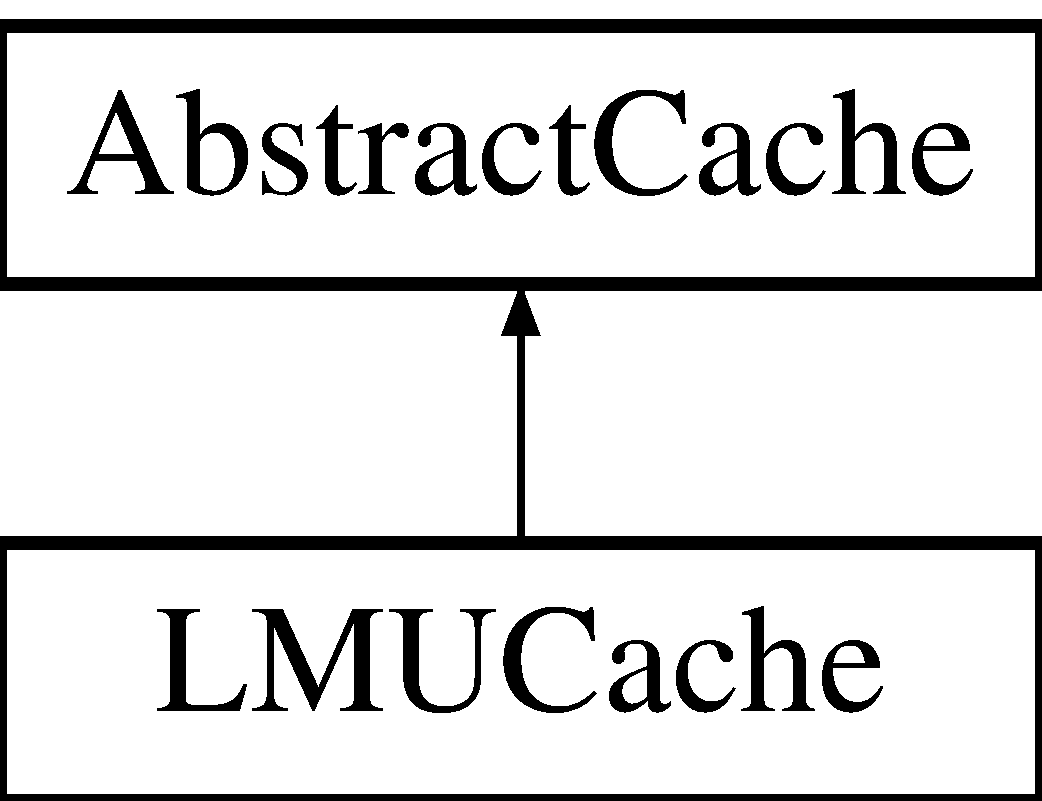
\includegraphics[height=2.000000cm]{classLMUCache}
\end{center}
\end{figure}
\subsection*{\-Public \-Member \-Functions}
\begin{DoxyCompactItemize}
\item 
\hypertarget{classLMUCache_a315045011c84226323bc88f52628d910}{\hyperlink{classLMUCache_a315045011c84226323bc88f52628d910}{\-L\-M\-U\-Cache} ()}\label{classLMUCache_a315045011c84226323bc88f52628d910}

\begin{DoxyCompactList}\small\item\em \-L\-M\-U \-Constructor. \end{DoxyCompactList}\item 
\hypertarget{classLMUCache_a59889726c35a2f2a6f6b873f94dd2e87}{\hyperlink{classLMUCache_a59889726c35a2f2a6f6b873f94dd2e87}{$\sim$\-L\-M\-U\-Cache} ()}\label{classLMUCache_a59889726c35a2f2a6f6b873f94dd2e87}

\begin{DoxyCompactList}\small\item\em \-L\-M\-U \-Destructor. \end{DoxyCompactList}\item 
void \hyperlink{classLMUCache_a00f0c220918265d669ae49eb71b179a9}{update\-List} (string url)
\begin{DoxyCompactList}\small\item\em \-Update the \-List. \end{DoxyCompactList}\item 
int \hyperlink{classLMUCache_abe671d7cb4d2fa3455fca1d4e2d9a8a4}{pick\-Index\-For\-Next\-Deletion} ()
\begin{DoxyCompactList}\small\item\em \-Select \-Next \-Candidate for \-Eviction. \end{DoxyCompactList}\item 
void \hyperlink{classLMUCache_aa284a631c7725948fdcfe9715ad4b420}{insert\-Into\-List} (string url, string content)
\begin{DoxyCompactList}\small\item\em \-Insert \-U\-R\-L to back of the \-Queue. \end{DoxyCompactList}\end{DoxyCompactItemize}


\subsection{\-Detailed \-Description}
\hyperlink{classLMUCache}{\-L\-M\-U\-Cache}. 

\subsection{\-Member \-Function \-Documentation}
\hypertarget{classLMUCache_aa284a631c7725948fdcfe9715ad4b420}{\index{\-L\-M\-U\-Cache@{\-L\-M\-U\-Cache}!insert\-Into\-List@{insert\-Into\-List}}
\index{insert\-Into\-List@{insert\-Into\-List}!LMUCache@{\-L\-M\-U\-Cache}}
\subsubsection[{insert\-Into\-List}]{\setlength{\rightskip}{0pt plus 5cm}void {\bf \-L\-M\-U\-Cache\-::insert\-Into\-List} (
\begin{DoxyParamCaption}
\item[{string}]{url, }
\item[{string}]{content}
\end{DoxyParamCaption}
)\hspace{0.3cm}{\ttfamily  \mbox{[}virtual\mbox{]}}}}\label{classLMUCache_aa284a631c7725948fdcfe9715ad4b420}


\-Insert \-U\-R\-L to back of the \-Queue. 


\begin{DoxyParams}{\-Parameters}
{\em url} & \\
\hline
{\em content} & -\/ \-Web \-Content \\
\hline
\end{DoxyParams}
\begin{DoxyReturn}{\-Returns}
none 
\end{DoxyReturn}


\-Implements \hyperlink{classAbstractCache}{\-Abstract\-Cache}.

\hypertarget{classLMUCache_abe671d7cb4d2fa3455fca1d4e2d9a8a4}{\index{\-L\-M\-U\-Cache@{\-L\-M\-U\-Cache}!pick\-Index\-For\-Next\-Deletion@{pick\-Index\-For\-Next\-Deletion}}
\index{pick\-Index\-For\-Next\-Deletion@{pick\-Index\-For\-Next\-Deletion}!LMUCache@{\-L\-M\-U\-Cache}}
\subsubsection[{pick\-Index\-For\-Next\-Deletion}]{\setlength{\rightskip}{0pt plus 5cm}int {\bf \-L\-M\-U\-Cache\-::pick\-Index\-For\-Next\-Deletion} (
\begin{DoxyParamCaption}
{}
\end{DoxyParamCaption}
)\hspace{0.3cm}{\ttfamily  \mbox{[}virtual\mbox{]}}}}\label{classLMUCache_abe671d7cb4d2fa3455fca1d4e2d9a8a4}


\-Select \-Next \-Candidate for \-Eviction. 

\begin{DoxyReturn}{\-Returns}
index of next candidate for eviction 
\end{DoxyReturn}


\-Implements \hyperlink{classAbstractCache}{\-Abstract\-Cache}.

\hypertarget{classLMUCache_a00f0c220918265d669ae49eb71b179a9}{\index{\-L\-M\-U\-Cache@{\-L\-M\-U\-Cache}!update\-List@{update\-List}}
\index{update\-List@{update\-List}!LMUCache@{\-L\-M\-U\-Cache}}
\subsubsection[{update\-List}]{\setlength{\rightskip}{0pt plus 5cm}void {\bf \-L\-M\-U\-Cache\-::update\-List} (
\begin{DoxyParamCaption}
\item[{string}]{url}
\end{DoxyParamCaption}
)\hspace{0.3cm}{\ttfamily  \mbox{[}virtual\mbox{]}}}}\label{classLMUCache_a00f0c220918265d669ae49eb71b179a9}


\-Update the \-List. 

\begin{DoxyAuthor}{\-Author}
\-Akshata \-Rao 
\end{DoxyAuthor}

\begin{DoxyParams}{\-Parameters}
{\em url} & -\/ \-U\-R\-L \\
\hline
\end{DoxyParams}
\begin{DoxyReturn}{\-Returns}
none 
\end{DoxyReturn}


\-Implements \hyperlink{classAbstractCache}{\-Abstract\-Cache}.



\-The documentation for this class was generated from the following files\-:\begin{DoxyCompactItemize}
\item 
\hyperlink{LMUCache_8h}{\-L\-M\-U\-Cache.\-h}\item 
\hyperlink{LMUCache_8cpp}{\-L\-M\-U\-Cache.\-cpp}\end{DoxyCompactItemize}

\hypertarget{classLRUCache}{\section{\-L\-R\-U\-Cache \-Class \-Reference}
\label{classLRUCache}\index{\-L\-R\-U\-Cache@{\-L\-R\-U\-Cache}}
}


\hyperlink{classLRUCache}{\-L\-R\-U\-Cache}.  




{\ttfamily \#include $<$\-L\-R\-U\-Cache.\-h$>$}

\-Inheritance diagram for \-L\-R\-U\-Cache\-:\begin{figure}[H]
\begin{center}
\leavevmode
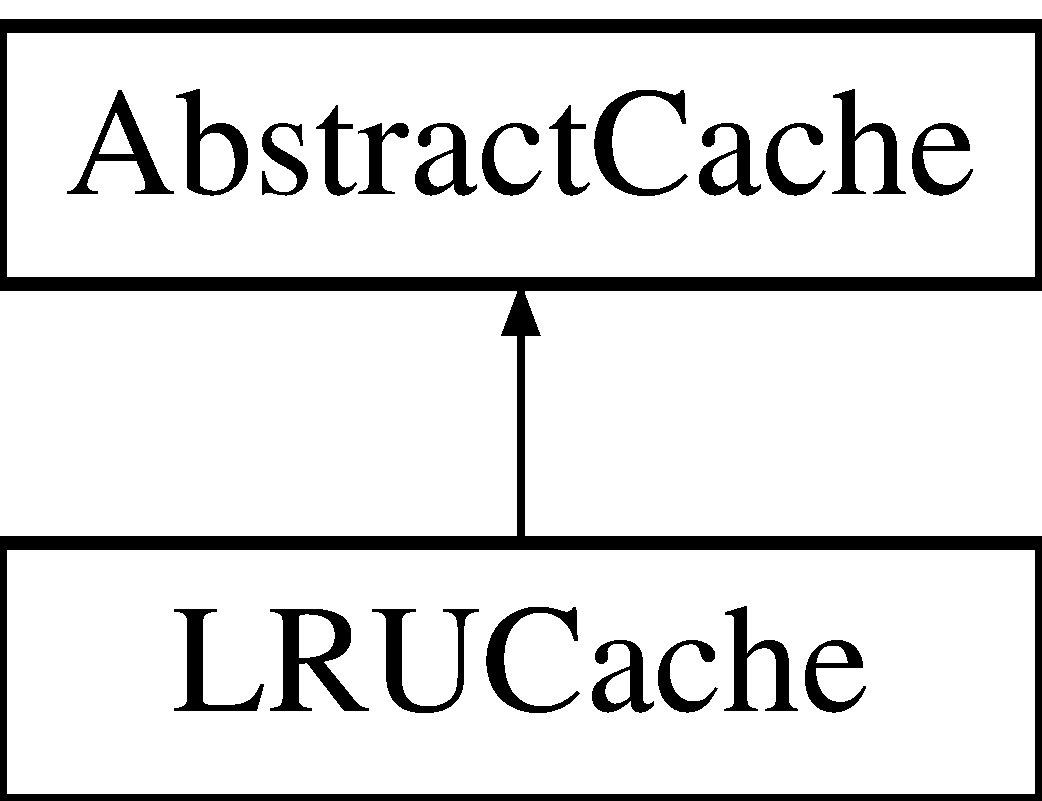
\includegraphics[height=2.000000cm]{classLRUCache}
\end{center}
\end{figure}
\subsection*{\-Public \-Member \-Functions}
\begin{DoxyCompactItemize}
\item 
\hyperlink{classLRUCache_a6f624ad11516bc5c8b56ab19250902bb}{\-L\-R\-U\-Cache} ()
\begin{DoxyCompactList}\small\item\em constructor \end{DoxyCompactList}\item 
\hyperlink{classLRUCache_ac841ed5b67e603f2878c26ea7555385f}{$\sim$\-L\-R\-U\-Cache} ()
\begin{DoxyCompactList}\small\item\em destructor \end{DoxyCompactList}\item 
void \hyperlink{classLRUCache_a9ade7fe6ec5353a5b4259ad48929122b}{update\-List} (string url)
\begin{DoxyCompactList}\small\item\em \-Update the \-Candidate \-Queue with \-U\-R\-L. \end{DoxyCompactList}\item 
int \hyperlink{classLRUCache_ab5e4e2db90274ce42e32f0ea466db0ef}{pick\-Index\-For\-Next\-Deletion} ()
\begin{DoxyCompactList}\small\item\em \-Select the next candidate for eviction. \end{DoxyCompactList}\item 
void \hyperlink{classLRUCache_aa767d58be45c61f2e9a1073343465e16}{insert\-Into\-List} (string url, string content)
\begin{DoxyCompactList}\small\item\em \-Insert the web content eviction candidate into queue. \end{DoxyCompactList}\end{DoxyCompactItemize}


\subsection{\-Detailed \-Description}
\hyperlink{classLRUCache}{\-L\-R\-U\-Cache}. 

\subsection{\-Constructor \& \-Destructor \-Documentation}
\hypertarget{classLRUCache_a6f624ad11516bc5c8b56ab19250902bb}{\index{\-L\-R\-U\-Cache@{\-L\-R\-U\-Cache}!\-L\-R\-U\-Cache@{\-L\-R\-U\-Cache}}
\index{\-L\-R\-U\-Cache@{\-L\-R\-U\-Cache}!LRUCache@{\-L\-R\-U\-Cache}}
\subsubsection[{\-L\-R\-U\-Cache}]{\setlength{\rightskip}{0pt plus 5cm}{\bf \-L\-R\-U\-Cache\-::\-L\-R\-U\-Cache} (
\begin{DoxyParamCaption}
{}
\end{DoxyParamCaption}
)}}\label{classLRUCache_a6f624ad11516bc5c8b56ab19250902bb}


constructor 

\-L\-R\-U \-Constructor. \hypertarget{classLRUCache_ac841ed5b67e603f2878c26ea7555385f}{\index{\-L\-R\-U\-Cache@{\-L\-R\-U\-Cache}!$\sim$\-L\-R\-U\-Cache@{$\sim$\-L\-R\-U\-Cache}}
\index{$\sim$\-L\-R\-U\-Cache@{$\sim$\-L\-R\-U\-Cache}!LRUCache@{\-L\-R\-U\-Cache}}
\subsubsection[{$\sim$\-L\-R\-U\-Cache}]{\setlength{\rightskip}{0pt plus 5cm}{\bf \-L\-R\-U\-Cache\-::$\sim$\-L\-R\-U\-Cache} (
\begin{DoxyParamCaption}
{}
\end{DoxyParamCaption}
)}}\label{classLRUCache_ac841ed5b67e603f2878c26ea7555385f}


destructor 

\-L\-R\-U \-Destructor. 

\subsection{\-Member \-Function \-Documentation}
\hypertarget{classLRUCache_aa767d58be45c61f2e9a1073343465e16}{\index{\-L\-R\-U\-Cache@{\-L\-R\-U\-Cache}!insert\-Into\-List@{insert\-Into\-List}}
\index{insert\-Into\-List@{insert\-Into\-List}!LRUCache@{\-L\-R\-U\-Cache}}
\subsubsection[{insert\-Into\-List}]{\setlength{\rightskip}{0pt plus 5cm}void {\bf \-L\-R\-U\-Cache\-::insert\-Into\-List} (
\begin{DoxyParamCaption}
\item[{string}]{url, }
\item[{string}]{content}
\end{DoxyParamCaption}
)\hspace{0.3cm}{\ttfamily  \mbox{[}virtual\mbox{]}}}}\label{classLRUCache_aa767d58be45c61f2e9a1073343465e16}


\-Insert the web content eviction candidate into queue. 

\-Insert \-U\-R\-L to back of the \-Queue.


\begin{DoxyParams}{\-Parameters}
{\em url} & \\
\hline
{\em content} & -\/ \-Web \-Content \\
\hline
\end{DoxyParams}
\begin{DoxyReturn}{\-Returns}
none 
\end{DoxyReturn}


\-Implements \hyperlink{classAbstractCache_a910756174d1ee21eac16a4be3f7c881a}{\-Abstract\-Cache}.

\hypertarget{classLRUCache_ab5e4e2db90274ce42e32f0ea466db0ef}{\index{\-L\-R\-U\-Cache@{\-L\-R\-U\-Cache}!pick\-Index\-For\-Next\-Deletion@{pick\-Index\-For\-Next\-Deletion}}
\index{pick\-Index\-For\-Next\-Deletion@{pick\-Index\-For\-Next\-Deletion}!LRUCache@{\-L\-R\-U\-Cache}}
\subsubsection[{pick\-Index\-For\-Next\-Deletion}]{\setlength{\rightskip}{0pt plus 5cm}int {\bf \-L\-R\-U\-Cache\-::pick\-Index\-For\-Next\-Deletion} (
\begin{DoxyParamCaption}
{}
\end{DoxyParamCaption}
)\hspace{0.3cm}{\ttfamily  \mbox{[}virtual\mbox{]}}}}\label{classLRUCache_ab5e4e2db90274ce42e32f0ea466db0ef}


\-Select the next candidate for eviction. 

\-Select \-Next \-Candidate for \-Eviction.

\begin{DoxyReturn}{\-Returns}
index of next candidate for eviction 
\end{DoxyReturn}


\-Implements \hyperlink{classAbstractCache_ae9fe168b0b9167c27b94b4a3a1be788c}{\-Abstract\-Cache}.

\hypertarget{classLRUCache_a9ade7fe6ec5353a5b4259ad48929122b}{\index{\-L\-R\-U\-Cache@{\-L\-R\-U\-Cache}!update\-List@{update\-List}}
\index{update\-List@{update\-List}!LRUCache@{\-L\-R\-U\-Cache}}
\subsubsection[{update\-List}]{\setlength{\rightskip}{0pt plus 5cm}void {\bf \-L\-R\-U\-Cache\-::update\-List} (
\begin{DoxyParamCaption}
\item[{string}]{url}
\end{DoxyParamCaption}
)\hspace{0.3cm}{\ttfamily  \mbox{[}virtual\mbox{]}}}}\label{classLRUCache_a9ade7fe6ec5353a5b4259ad48929122b}


\-Update the \-Candidate \-Queue with \-U\-R\-L. 

\-Update the \-List.

\begin{DoxyAuthor}{\-Author}
\-Spoorthi \-Ravi 
\end{DoxyAuthor}

\begin{DoxyParams}{\-Parameters}
{\em url} & -\/ \-U\-R\-L \\
\hline
\end{DoxyParams}
\begin{DoxyReturn}{\-Returns}
none 
\end{DoxyReturn}


\-Implements \hyperlink{classAbstractCache_a67552fbca85ce7dbc7e2c553b1036884}{\-Abstract\-Cache}.



\-The documentation for this class was generated from the following files\-:\begin{DoxyCompactItemize}
\item 
\hyperlink{LRUCache_8h}{\-L\-R\-U\-Cache.\-h}\item 
\hyperlink{LRUCache_8cpp}{\-L\-R\-U\-Cache.\-cpp}\end{DoxyCompactItemize}

\hypertarget{classRandomCache}{\section{\-Random\-Cache \-Class \-Reference}
\label{classRandomCache}\index{\-Random\-Cache@{\-Random\-Cache}}
}


\hyperlink{classRandomCache}{\-Random\-Cache}.  




{\ttfamily \#include $<$\-Random\-Cache.\-h$>$}

\-Inheritance diagram for \-Random\-Cache\-:\begin{figure}[H]
\begin{center}
\leavevmode
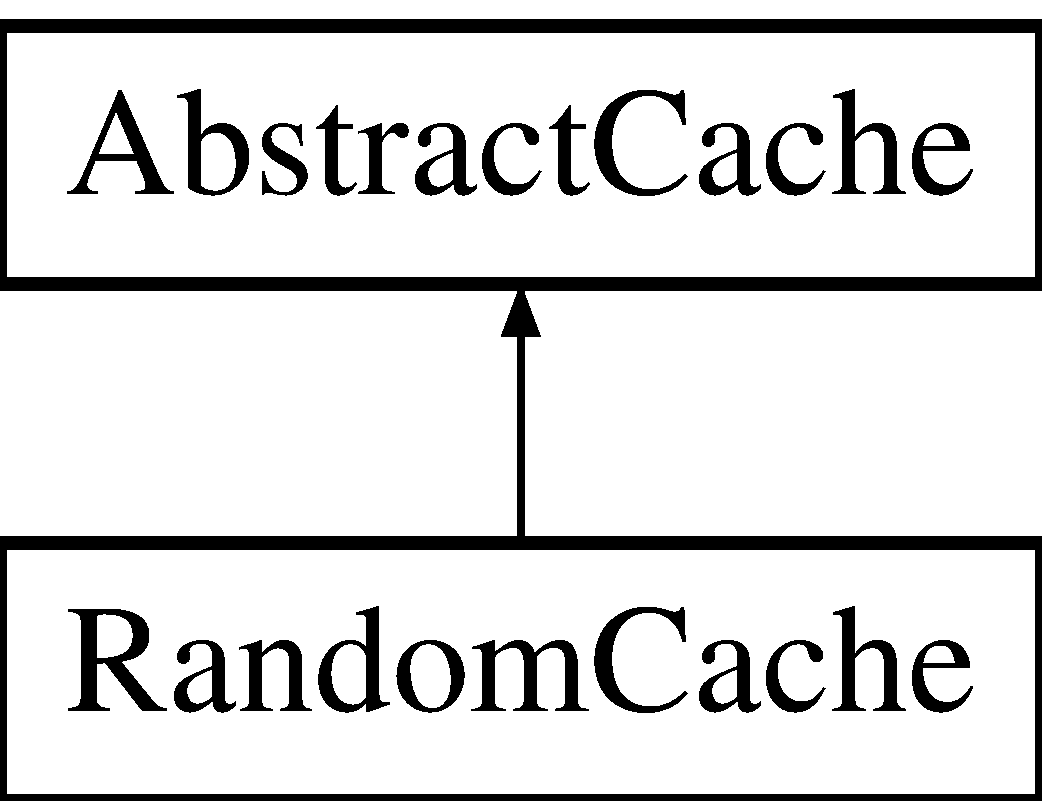
\includegraphics[height=2.000000cm]{classRandomCache}
\end{center}
\end{figure}
\subsection*{\-Public \-Member \-Functions}
\begin{DoxyCompactItemize}
\item 
\hypertarget{classRandomCache_ac8fc4e9935427c8e05ae6bb01322654d}{\hyperlink{classRandomCache_ac8fc4e9935427c8e05ae6bb01322654d}{$\sim$\-Random\-Cache} ()}\label{classRandomCache_ac8fc4e9935427c8e05ae6bb01322654d}

\begin{DoxyCompactList}\small\item\em \-Random \-Cache \-Destructor. \end{DoxyCompactList}\item 
\hypertarget{classRandomCache_a1e619bf1789ec07f0ab622f559dbb52a}{\hyperlink{classRandomCache_a1e619bf1789ec07f0ab622f559dbb52a}{\-Random\-Cache} ()}\label{classRandomCache_a1e619bf1789ec07f0ab622f559dbb52a}

\begin{DoxyCompactList}\small\item\em \-Random \-Cache \-Constructor. \end{DoxyCompactList}\item 
void \hyperlink{classRandomCache_a3aae77b7542e80418669d138223cfcc0}{update\-List} (string url)
\begin{DoxyCompactList}\small\item\em \-Update the \-Queue. \end{DoxyCompactList}\item 
int \hyperlink{classRandomCache_ad9362f5b0a972495d03beca2c770d10b}{pick\-Index\-For\-Next\-Deletion} ()
\begin{DoxyCompactList}\small\item\em \-Select next candidate for eviction. \end{DoxyCompactList}\item 
void \hyperlink{classRandomCache_aac3ac982daf70108b6b179bb0cdb787d}{insert\-Into\-List} (string url, string content)
\begin{DoxyCompactList}\small\item\em \-Insert \-U\-R\-L to back of the \-Queue. \end{DoxyCompactList}\end{DoxyCompactItemize}


\subsection{\-Detailed \-Description}
\hyperlink{classRandomCache}{\-Random\-Cache}. 

\subsection{\-Member \-Function \-Documentation}
\hypertarget{classRandomCache_aac3ac982daf70108b6b179bb0cdb787d}{\index{\-Random\-Cache@{\-Random\-Cache}!insert\-Into\-List@{insert\-Into\-List}}
\index{insert\-Into\-List@{insert\-Into\-List}!RandomCache@{\-Random\-Cache}}
\subsubsection[{insert\-Into\-List}]{\setlength{\rightskip}{0pt plus 5cm}void {\bf \-Random\-Cache\-::insert\-Into\-List} (
\begin{DoxyParamCaption}
\item[{string}]{url, }
\item[{string}]{content}
\end{DoxyParamCaption}
)\hspace{0.3cm}{\ttfamily  \mbox{[}virtual\mbox{]}}}}\label{classRandomCache_aac3ac982daf70108b6b179bb0cdb787d}


\-Insert \-U\-R\-L to back of the \-Queue. 


\begin{DoxyParams}{\-Parameters}
{\em url} & \\
\hline
{\em content} & -\/ \-Web \-Content \\
\hline
\end{DoxyParams}
\begin{DoxyReturn}{\-Returns}
none 
\end{DoxyReturn}


\-Implements \hyperlink{classAbstractCache_a910756174d1ee21eac16a4be3f7c881a}{\-Abstract\-Cache}.

\hypertarget{classRandomCache_ad9362f5b0a972495d03beca2c770d10b}{\index{\-Random\-Cache@{\-Random\-Cache}!pick\-Index\-For\-Next\-Deletion@{pick\-Index\-For\-Next\-Deletion}}
\index{pick\-Index\-For\-Next\-Deletion@{pick\-Index\-For\-Next\-Deletion}!RandomCache@{\-Random\-Cache}}
\subsubsection[{pick\-Index\-For\-Next\-Deletion}]{\setlength{\rightskip}{0pt plus 5cm}int {\bf \-Random\-Cache\-::pick\-Index\-For\-Next\-Deletion} (
\begin{DoxyParamCaption}
{}
\end{DoxyParamCaption}
)\hspace{0.3cm}{\ttfamily  \mbox{[}virtual\mbox{]}}}}\label{classRandomCache_ad9362f5b0a972495d03beca2c770d10b}


\-Select next candidate for eviction. 

\begin{DoxyReturn}{\-Returns}
\-Index for candidate for eviction 
\end{DoxyReturn}


\-Implements \hyperlink{classAbstractCache_ae9fe168b0b9167c27b94b4a3a1be788c}{\-Abstract\-Cache}.

\hypertarget{classRandomCache_a3aae77b7542e80418669d138223cfcc0}{\index{\-Random\-Cache@{\-Random\-Cache}!update\-List@{update\-List}}
\index{update\-List@{update\-List}!RandomCache@{\-Random\-Cache}}
\subsubsection[{update\-List}]{\setlength{\rightskip}{0pt plus 5cm}void {\bf \-Random\-Cache\-::update\-List} (
\begin{DoxyParamCaption}
\item[{string}]{url}
\end{DoxyParamCaption}
)\hspace{0.3cm}{\ttfamily  \mbox{[}virtual\mbox{]}}}}\label{classRandomCache_a3aae77b7542e80418669d138223cfcc0}


\-Update the \-Queue. 

\begin{DoxyAuthor}{\-Author}
\-Akshata \-Rao 
\end{DoxyAuthor}

\begin{DoxyParams}{\-Parameters}
{\em \-U\-R\-L} & \\
\hline
\end{DoxyParams}
\begin{DoxyReturn}{\-Returns}
none 
\end{DoxyReturn}


\-Implements \hyperlink{classAbstractCache_a67552fbca85ce7dbc7e2c553b1036884}{\-Abstract\-Cache}.



\-The documentation for this class was generated from the following files\-:\begin{DoxyCompactItemize}
\item 
\hyperlink{RandomCache_8h}{\-Random\-Cache.\-h}\item 
\hyperlink{RandomCache_8cpp}{\-Random\-Cache.\-cpp}\end{DoxyCompactItemize}

\hypertarget{classRPCProxyHandler}{\section{\-R\-P\-C\-Proxy\-Handler \-Class \-Reference}
\label{classRPCProxyHandler}\index{\-R\-P\-C\-Proxy\-Handler@{\-R\-P\-C\-Proxy\-Handler}}
}



\begin{DoxyItemize}
\item \hyperlink{classRPCProxyHandler}{\-R\-P\-C\-Proxy\-Handler} 
\end{DoxyItemize} 


\subsection*{\-Public \-Member \-Functions}
\begin{DoxyCompactItemize}
\item 
\hypertarget{classRPCProxyHandler_a410b74fb33e3d8f86c6ef441eb3e941f}{\hyperlink{classRPCProxyHandler_a410b74fb33e3d8f86c6ef441eb3e941f}{\-R\-P\-C\-Proxy\-Handler} ()}\label{classRPCProxyHandler_a410b74fb33e3d8f86c6ef441eb3e941f}

\begin{DoxyCompactList}\small\item\em \-Constructor. \end{DoxyCompactList}\item 
\hypertarget{classRPCProxyHandler_a13211f85624d234a58ece66412f845ab}{void {\bfseries hello} ()}\label{classRPCProxyHandler_a13211f85624d234a58ece66412f845ab}

\item 
void \hyperlink{classRPCProxyHandler_a4b821c2866975f9d686e830df86095a4}{fetch\-U\-R\-L\-Content} (std\-::string \&\-\_\-return, const std\-::string \&url)
\begin{DoxyCompactList}\small\item\em \-Fetch \-Web \-Content for given \-U\-R\-L. \end{DoxyCompactList}\item 
\hypertarget{classRPCProxyHandler_ab02e49e5ab6b7c8e83ff3c411a5ff0f4}{void {\bfseries print\-Server\-Stats} ()}\label{classRPCProxyHandler_ab02e49e5ab6b7c8e83ff3c411a5ff0f4}

\end{DoxyCompactItemize}
\subsection*{\-Static \-Public \-Member \-Functions}
\begin{DoxyCompactItemize}
\item 
\hypertarget{classRPCProxyHandler_a4502c256cc2202280a3626080d2cc3ab}{static size\-\_\-t {\bfseries \-Write\-Callback} (void $\ast$contents, size\-\_\-t size, size\-\_\-t nmemb, void $\ast$userp)}\label{classRPCProxyHandler_a4502c256cc2202280a3626080d2cc3ab}

\end{DoxyCompactItemize}
\subsection*{\-Public \-Attributes}
\begin{DoxyCompactItemize}
\item 
\hypertarget{classRPCProxyHandler_a2ac0df19d0b5b6f486593886f281cc37}{int {\bfseries number\-Of\-Requests}}\label{classRPCProxyHandler_a2ac0df19d0b5b6f486593886f281cc37}

\item 
\hypertarget{classRPCProxyHandler_a584e1d2460a6d189e7830226d0d48ed3}{double {\bfseries total\-Time}}\label{classRPCProxyHandler_a584e1d2460a6d189e7830226d0d48ed3}

\item 
\hypertarget{classRPCProxyHandler_a382e5666620ce07bdd771f62c2494110}{int {\bfseries cache\-Hits}}\label{classRPCProxyHandler_a382e5666620ce07bdd771f62c2494110}

\item 
\hypertarget{classRPCProxyHandler_a647a7727373b329adc985b59ca2710d5}{int {\bfseries cache\-Rejections}}\label{classRPCProxyHandler_a647a7727373b329adc985b59ca2710d5}

\item 
\hypertarget{classRPCProxyHandler_a75985d9116b06d96c6e7e23c10e1c12e}{int {\bfseries cache\-Misses}}\label{classRPCProxyHandler_a75985d9116b06d96c6e7e23c10e1c12e}

\end{DoxyCompactItemize}


\subsection{\-Detailed \-Description}

\begin{DoxyItemize}
\item \hyperlink{classRPCProxyHandler}{\-R\-P\-C\-Proxy\-Handler} 
\end{DoxyItemize}

\subsection{\-Member \-Function \-Documentation}
\hypertarget{classRPCProxyHandler_a4b821c2866975f9d686e830df86095a4}{\index{\-R\-P\-C\-Proxy\-Handler@{\-R\-P\-C\-Proxy\-Handler}!fetch\-U\-R\-L\-Content@{fetch\-U\-R\-L\-Content}}
\index{fetch\-U\-R\-L\-Content@{fetch\-U\-R\-L\-Content}!RPCProxyHandler@{\-R\-P\-C\-Proxy\-Handler}}
\subsubsection[{fetch\-U\-R\-L\-Content}]{\setlength{\rightskip}{0pt plus 5cm}void {\bf \-R\-P\-C\-Proxy\-Handler\-::fetch\-U\-R\-L\-Content} (
\begin{DoxyParamCaption}
\item[{std\-::string \&}]{\-\_\-return, }
\item[{const std\-::string \&}]{url}
\end{DoxyParamCaption}
)\hspace{0.3cm}{\ttfamily  \mbox{[}inline\mbox{]}}}}\label{classRPCProxyHandler_a4b821c2866975f9d686e830df86095a4}


\-Fetch \-Web \-Content for given \-U\-R\-L. 


\begin{DoxyParams}{\-Parameters}
{\em \-\_\-return} & -\/ \-Web \-Content is saved here \\
\hline
{\em url} & -\/ \-U\-R\-L \\
\hline
\end{DoxyParams}
\begin{DoxyReturn}{\-Returns}
-\/ none 
\end{DoxyReturn}


\-The documentation for this class was generated from the following file\-:\begin{DoxyCompactItemize}
\item 
\-R\-P\-C\-Proxy\-Server.\-cpp\end{DoxyCompactItemize}

\hypertarget{classURLNode}{\section{\-U\-R\-L\-Node \-Struct \-Reference}
\label{classURLNode}\index{\-U\-R\-L\-Node@{\-U\-R\-L\-Node}}
}
\subsection*{\-Public \-Member \-Functions}
\begin{DoxyCompactItemize}
\item 
\hyperlink{classURLNode_a884b929b580ed24de145730114e45f01}{\-U\-R\-L\-Node} (string url\-Input, string content\-Input)
\begin{DoxyCompactList}\small\item\em \hyperlink{classURLNode}{\-U\-R\-L\-Node} \-Constructor. \end{DoxyCompactList}\end{DoxyCompactItemize}
\subsection*{\-Public \-Attributes}
\begin{DoxyCompactItemize}
\item 
\hypertarget{classURLNode_a56a91b8a8ce53f8f18eb084aa819f0b1}{string \hyperlink{classURLNode_a56a91b8a8ce53f8f18eb084aa819f0b1}{url}}\label{classURLNode_a56a91b8a8ce53f8f18eb084aa819f0b1}

\begin{DoxyCompactList}\small\item\em \-U\-R\-L. \end{DoxyCompactList}\item 
\hypertarget{classURLNode_ab3472b86fa6d65fe261cfba0f87afac4}{string \hyperlink{classURLNode_ab3472b86fa6d65fe261cfba0f87afac4}{content}}\label{classURLNode_ab3472b86fa6d65fe261cfba0f87afac4}

\begin{DoxyCompactList}\small\item\em \-Web \-Content. \end{DoxyCompactList}\item 
\hypertarget{classURLNode_ac71b006475d8b170f19110783451c5a7}{int \hyperlink{classURLNode_ac71b006475d8b170f19110783451c5a7}{content\-Size}}\label{classURLNode_ac71b006475d8b170f19110783451c5a7}

\begin{DoxyCompactList}\small\item\em \-Content \-Size. \end{DoxyCompactList}\item 
\hypertarget{classURLNode_a8668b5a701d39dde07f171c987233343}{struct \hyperlink{classURLNode}{\-U\-R\-L\-Node} $\ast$ {\bfseries left}}\label{classURLNode_a8668b5a701d39dde07f171c987233343}

\item 
\hypertarget{classURLNode_ac7246d0b922dad7c70dc74088de96c5b}{struct \hyperlink{classURLNode}{\-U\-R\-L\-Node} $\ast$ {\bfseries right}}\label{classURLNode_ac7246d0b922dad7c70dc74088de96c5b}

\item 
\hypertarget{classURLNode_ad682feead55da0df4f4630a41bcaa025}{const char $\ast$ {\bfseries url}}\label{classURLNode_ad682feead55da0df4f4630a41bcaa025}

\item 
\hypertarget{classURLNode_aab5544f645e09fd251094437376d4397}{const char $\ast$ {\bfseries content}}\label{classURLNode_aab5544f645e09fd251094437376d4397}

\end{DoxyCompactItemize}


\subsection{\-Constructor \& \-Destructor \-Documentation}
\hypertarget{classURLNode_a884b929b580ed24de145730114e45f01}{\index{\-U\-R\-L\-Node@{\-U\-R\-L\-Node}!\-U\-R\-L\-Node@{\-U\-R\-L\-Node}}
\index{\-U\-R\-L\-Node@{\-U\-R\-L\-Node}!URLNode@{\-U\-R\-L\-Node}}
\subsubsection[{\-U\-R\-L\-Node}]{\setlength{\rightskip}{0pt plus 5cm}{\bf \-U\-R\-L\-Node\-::\-U\-R\-L\-Node} (
\begin{DoxyParamCaption}
\item[{string}]{url\-Input, }
\item[{string}]{content\-Input}
\end{DoxyParamCaption}
)\hspace{0.3cm}{\ttfamily  \mbox{[}inline\mbox{]}}}}\label{classURLNode_a884b929b580ed24de145730114e45f01}


\hyperlink{classURLNode}{\-U\-R\-L\-Node} \-Constructor. 

\-Sets the \-U\-R\-L and webcontent for each node 

\-The documentation for this struct was generated from the following files\-:\begin{DoxyCompactItemize}
\item 
\hyperlink{AbstractCache_8h}{\-Abstract\-Cache.\-h}\item 
\-U\-R\-L\-Search\-Tree.\-cpp\end{DoxyCompactItemize}

\chapter{\-File \-Documentation}
\hypertarget{AbstractCache_8cpp}{\section{\-Abstract\-Cache.\-cpp \-File \-Reference}
\label{AbstractCache_8cpp}\index{\-Abstract\-Cache.\-cpp@{\-Abstract\-Cache.\-cpp}}
}
{\ttfamily \#include \char`\"{}\-Abstract\-Cache.\-h\char`\"{}}\*
{\ttfamily \#include $<$iostream$>$}\*


\subsection{\-Detailed \-Description}
\begin{DoxyAuthor}{\-Author}
\-Spoorthi \-Ravi 
\end{DoxyAuthor}

\hypertarget{AbstractCache_8h}{\section{\-Abstract\-Cache.\-h \-File \-Reference}
\label{AbstractCache_8h}\index{\-Abstract\-Cache.\-h@{\-Abstract\-Cache.\-h}}
}
{\ttfamily \#include $<$string$>$}\*
{\ttfamily \#include $<$vector$>$}\*
{\ttfamily \#include $<$unordered\-\_\-map$>$}\*
\subsection*{\-Classes}
\begin{DoxyCompactItemize}
\item 
struct \hyperlink{classURLNode}{\-U\-R\-L\-Node}
\item 
class \hyperlink{classAbstractCache}{\-Abstract\-Cache}
\end{DoxyCompactItemize}
\subsection*{\-Defines}
\begin{DoxyCompactItemize}
\item 
\hypertarget{AbstractCache_8h_a6c8469dfe973ac952cf40394bd2c160b}{\#define {\bfseries \-M\-A\-X\-\_\-\-C\-A\-C\-H\-E\-\_\-\-S\-I\-Z\-E}~20}\label{AbstractCache_8h_a6c8469dfe973ac952cf40394bd2c160b}

\end{DoxyCompactItemize}


\subsection{\-Detailed \-Description}
\begin{DoxyAuthor}{\-Author}
\-Spoorthi \-Ravi 
\end{DoxyAuthor}

\hypertarget{FIFOCache_8h}{\section{\-F\-I\-F\-O\-Cache.\-h \-File \-Reference}
\label{FIFOCache_8h}\index{\-F\-I\-F\-O\-Cache.\-h@{\-F\-I\-F\-O\-Cache.\-h}}
}
{\ttfamily \#include $<$string$>$}\*
{\ttfamily \#include $<$unordered\-\_\-map$>$}\*
{\ttfamily \#include $<$vector$>$}\*
{\ttfamily \#include \char`\"{}\-Abstract\-Cache.\-h\char`\"{}}\*
\subsection*{\-Classes}
\begin{DoxyCompactItemize}
\item 
class \hyperlink{classFIFOCache}{\-F\-I\-F\-O\-Cache}
\begin{DoxyCompactList}\small\item\em \hyperlink{classFIFOCache}{\-F\-I\-F\-O\-Cache}. \end{DoxyCompactList}\end{DoxyCompactItemize}


\subsection{\-Detailed \-Description}

\hypertarget{LMUCache_8cpp}{\section{\-L\-M\-U\-Cache.\-cpp \-File \-Reference}
\label{LMUCache_8cpp}\index{\-L\-M\-U\-Cache.\-cpp@{\-L\-M\-U\-Cache.\-cpp}}
}
{\ttfamily \#include \char`\"{}\-L\-M\-U\-Cache.\-h\char`\"{}}\*
{\ttfamily \#include $<$iostream$>$}\*
{\ttfamily \#include $<$cstring$>$}\*


\subsection{\-Detailed \-Description}

\hypertarget{LMUCache_8h}{\section{\-L\-M\-U\-Cache.\-h \-File \-Reference}
\label{LMUCache_8h}\index{\-L\-M\-U\-Cache.\-h@{\-L\-M\-U\-Cache.\-h}}
}
{\ttfamily \#include $<$string$>$}\*
{\ttfamily \#include \char`\"{}\-Abstract\-Cache.\-h\char`\"{}}\*
\subsection*{\-Classes}
\begin{DoxyCompactItemize}
\item 
class \hyperlink{classLMUCache}{\-L\-M\-U\-Cache}
\begin{DoxyCompactList}\small\item\em \hyperlink{classLMUCache}{\-L\-M\-U\-Cache}. \end{DoxyCompactList}\end{DoxyCompactItemize}


\subsection{\-Detailed \-Description}
\begin{DoxyAuthor}{\-Author}
\-Akshata \-Rao 
\end{DoxyAuthor}

\hypertarget{LRUCache_8cpp}{\section{\-L\-R\-U\-Cache.\-cpp \-File \-Reference}
\label{LRUCache_8cpp}\index{\-L\-R\-U\-Cache.\-cpp@{\-L\-R\-U\-Cache.\-cpp}}
}
{\ttfamily \#include \char`\"{}\-L\-R\-U\-Cache.\-h\char`\"{}}\*
{\ttfamily \#include $<$iostream$>$}\*
{\ttfamily \#include $<$cstring$>$}\*


\subsection{\-Detailed \-Description}

\hypertarget{LRUCache_8h}{\section{\-L\-R\-U\-Cache.\-h \-File \-Reference}
\label{LRUCache_8h}\index{\-L\-R\-U\-Cache.\-h@{\-L\-R\-U\-Cache.\-h}}
}
{\ttfamily \#include $<$string$>$}\*
{\ttfamily \#include $<$unordered\-\_\-map$>$}\*
{\ttfamily \#include $<$vector$>$}\*
{\ttfamily \#include $<$algorithm$>$}\*
{\ttfamily \#include \char`\"{}\-Abstract\-Cache.\-h\char`\"{}}\*
\subsection*{\-Classes}
\begin{DoxyCompactItemize}
\item 
class \hyperlink{classLRUCache}{\-L\-R\-U\-Cache}
\begin{DoxyCompactList}\small\item\em \hyperlink{classLRUCache}{\-L\-R\-U\-Cache}. \end{DoxyCompactList}\end{DoxyCompactItemize}


\subsection{\-Detailed \-Description}
\begin{DoxyAuthor}{\-Author}
\-Spoorthi \-Ravi 
\end{DoxyAuthor}

\hypertarget{RandomCache_8h}{\section{\-Random\-Cache.\-h \-File \-Reference}
\label{RandomCache_8h}\index{\-Random\-Cache.\-h@{\-Random\-Cache.\-h}}
}
{\ttfamily \#include $<$string$>$}\*
{\ttfamily \#include $<$unordered\-\_\-map$>$}\*
{\ttfamily \#include $<$vector$>$}\*
{\ttfamily \#include \char`\"{}\-Abstract\-Cache.\-h\char`\"{}}\*
\subsection*{\-Classes}
\begin{DoxyCompactItemize}
\item 
class \hyperlink{classRandomCache}{\-Random\-Cache}
\begin{DoxyCompactList}\small\item\em \hyperlink{classRandomCache}{\-Random\-Cache}. \end{DoxyCompactList}\end{DoxyCompactItemize}


\subsection{\-Detailed \-Description}

\printindex
\end{document}
